\chapter{Relativistic Particles in Matter}
Neutrinos are notoriously difficult to detect. When high-energy neutrinos interact with matter, they produce secondary particles that travel fast enough to produce Cherenkov radiation. As indicated in section \ref{sec:detectors} cubic-sized experiments try to exploit this properties by using natural ice or water as the instrumented volume. In this chapter an overview of the behaviour of relativistic matter is given. The experiment that is used here is the IceCube detector, therefore there will be a larger focus on ice.

\section{Neutrino interactions}
\label{sec:neutrinointeractions}
Neutrino interactions with matter in both the charged current (CC) and neutral current (NC) interactions. In the former, the mediator particle is a charged W-boson resulting in a charged lepton in the final state. In the latter, the mediator particle is the neutral Z-boson. Both interaction types have a resulting hadronic component as daughter particles. The interactions can be written as

\begin{alignat}{2}
\nu_l \left(\bar{\nu}_l\right) + N &\xrightarrow{\text{W}^+} l^- \left(l^+\right) + X^{+\left(-\right)} \ \ && \left(CC\right)\\
\nu_l \left(\bar{\nu}_l\right) + N &\xrightarrow{\text{Z}} \nu'_l \left(\bar{\nu}'_l\right) + X && \left(NC\right),
\end{alignat}
where $l$ is the lepton flavor ($e,\mu,\tau$), $N$ denotes the inital hadronic state of the nucleus and $X$ the final hadronic state. These interactions are illustrated in Fig. \ref{fig:feynmanneutrino}.\\
\newline
The charged leptons and hadrons lead to light production via gamma ray production and Cherenkov radiation. With the right material it is possible to detect this light production and reconstruct some of the neutrino's characteristics.

\begin{figure}[t]
\label{fig:feynmanneutrino}
\centering
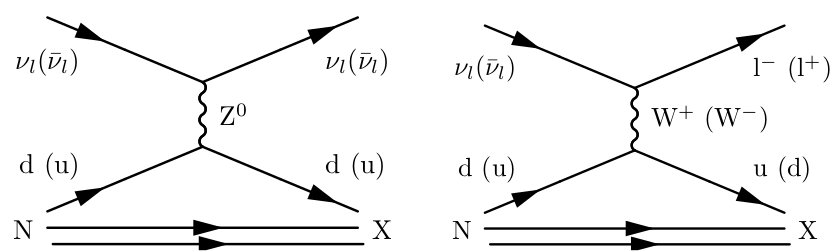
\includegraphics[width = 0.9\textwidth]{chapter4/img/feynmanneutrino.png}
\caption{Feynman diagrams of the NC (\textit{left}) and CC (\textit{right}) OVERAL SCHUINE LETTERS LINKSRECHTS? neutrino interactions. $l$ is the lepton flavor ($e,\mu,\tau$), $N$ denotes the inital hadronic state of the nucleus and $X$ the final hadronic state. The antineutrino interactions are given in between brackets.}
\end{figure}

\section{Cherenkov effect}
From Einstein's works on special and general relativity it follows that the speed of light in vacuum, $c$, is a universal constant. The speed of light in matter can be significantly lower than that. If a particle travels through a dielectric medium at a speed which is greater than the phase velocity of light in that medium, electromagnetic radiation is emitted. This radiation is called \textit{Cherenkov radiation} and is named after the first person who was able to detect it experimentally, Pavel Cherenkov. He was awarded the Nobel Prize in 1958 for his findings together with Frank and Tamm on their theoretical work on the subject \cite{nobel1958url}.

As can be seen in Appendix \cite{ch:planck}, equation \cite{eq:wave}, the velocity of a propagating wave is given by

\begin{equation}
\nabla^2\psi = \frac{1}{v^2} \frac{\partial \psi}{\partial t},
\end{equation}
where $\psi$ is the wave and $v$ it's group velocity. From Maxwell's equations and some vector calculus it is straightforward to find that the wave equation for electromagnetic radiation becomes

\begin{equation}
\nabla^2E = \mu \epsilon \frac{\partial E}{\partial t},
\end{equation}
where $E$ is the electric field and $\mu$ and $\epsilon$ the permeability and permittivity of the medium respectively. From these equations it is clear that for light in a dielectric medium

\begin{equation}
v = \frac{1}{\sqrt{\mu \epsilon}} = \frac{1}{\sqrt{\mu_r \epsilon_r}}\frac{1}{\sqrt{\mu_0 \epsilon_0}} = \frac{1}{\sqrt{\mu_r \epsilon_r}} \times c \leq c,
\end{equation}
where $1/\sqrt{\mu_0 \epsilon_0} = c$ and $\mu_r$ and $\epsilon_r$ are the relative (to vacuum) permeability and permittivity respectively and are $\geq 1$. These terms are also written as the refractive index $n = \sqrt{\mu_r \epsilon_r}$: $v = c/n$.

When a charged particle moves inside a dielectric medium, it excites the molecules of the medium to the higher levels and excited states. The molecules emit photons in the form of electromagnetic radiation upon returning back to their ground state. According to the \textit{Huygens principle}, the emitted waves move out spherically at the phase velocity of the medium (which can be less than the speed of light in vacuum). If the motion of the particle is slow, the radiated waves bunch up slightly in the direction of motion, but they do not cross. However if the particle moves faster than the light speed, the emitted waves add up constructively leading to a coherent radiation at angle $\theta_c$ with respect to the particle direction; Cherenkov radiation. The coherent interference is enough to be visible to the nnaked eye\footnote{The typical blue light in the cooling water at nuclear reactor sites is also due to this Cherenkov radiation.}. The signature of the effect is a cone of emission in the direction of particle motion. Fig. \ref{fig:cherenkov} shows a schematic of the Cherenkov radiation showing the typical spherical wavefront and the resultant radiation.

\begin{figure}[ht]
\label{fig:cherenkov}
\centering
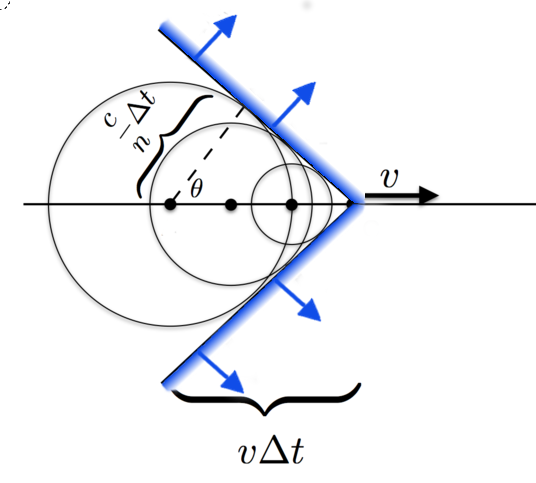
\includegraphics[width=0.6\textwidth]{chapter4/img/cherenkov2.png}
\caption{Schematic overview of Cherenkov radiation from a particle traveling at a velocity $v$.}
\end{figure}

From the figure we can derive that

\begin{equation}
\cos\theta_c = \frac{\frac{c}{n} \Delta t}{v \Delta t} = \frac{c}{vn} = \frac{1}{\beta n}.
\end{equation} 
Because $-1 \leq \cos\theta_c \leq 1$, the velocity of the charged particle must be $v \geq c/n$. Typical values of $n$ are on the order of 1-2, requiring the particles to be relativistic in order to emit Cherenkov radiation. The number of photons produced per unit path length of a particle with charge $ze$ and per unit energy interval of the photon was calculated by Frank and Tamm, and is often referred to as the Frank-Tamm equation

\begin{equation}
\begin{split}
\frac{d^2N}{dE dx} &= \frac{\alpha z^2}{\hbar c} \sin^2 \theta_c = \frac{\alpha^2 z^2}{r_e m_e c^2} \left( 1 - \frac{1}{\beta^2 n^2\left(E\right)} \right)\\
&\approx 370 \sin^2 \theta_c \left(E\right) \textrm{eV}^{-1} cm^{-1} \ \ \ \left( z =1\right),
\end{split}
\end{equation}
where $r_e$ is the classical electron radius, $m_e$ the electron mass and $\alpha$ the fine-structure constant. Equivalently, this equation can be written in function of the wavelength of the photon

\begin{equation}
\label{eq:franktamm}
\frac{d^2N}{dx d\lambda}  = \frac{2\pi \alpha z^2}{\lambda^2} \left(1- \frac{1}{\beta^2 n^2 \left(\lambda \right)} \right).
\end{equation}

As an example, air Cherenkov telescopes such as MAGIC, H.E.S.S and VERITAS look for the direct and indirect Cherenkov light from gamma rays and cosmic rays. Because the refractive index of air is close to 1 (1.000293 at sea level and smaller with increasing height) the opening angle of the Cherenkov cone is small ($\approx 1^{\circ}$). The particles need to be pretty relativistic in order for Cherenkov radiation to occur\footnote{Let us assume the refractive index of air at sea level, than from $E^2/m^2 = \gamma^2 = 1/(1-\beta^2)$ it follows the minimal energy is $\approx 41$ times it's rest mass. Since the refractive index decreases in function of height, the energies of particles interacting with the atmosphere must be even higher.}.

In water and ice, the refractive index is $\approx 1.33$, making $\beta_{min} = 0.75$ and $E_{min} = 1.51 \cdot m_0$. Experiments using water or ice as the interaction medium are Super-Kamiokande, ANTARES and the IceCube experiment.
\section{Propagation}
As described in section \ref{sec:neutrinointeractions}, neutrinos will give rise to several types of interactions in the surrounding medium. There are three characteristic signatures which are the main interest in the IceCube detector.

\subsection{Cascades}
A charged current neutrino interaction the energetic electron will give rise to a shower of gamma rays (bremsstrahlung), positrons and electrons (pair production). Positrons and electrons will in their turn emit new gamma rays and this process continues until the photon energies fall below the pair production threshold. Because electrons/positrons lose their energy fast, they are almost immediately stopped, giving an electromagnetic cascade a spherical shape. In the case of neutral current events, the breakup of the struck nucleus leads to charged byproducts. These byproducts can reinteract in the medium and produce neutral pions that decay into gamma rays. These particles again die out quickly, resulting in a spherical emission of light.

\subsubsection{Energy loss}
Er stond echt wel ergens iets, ook thesis nalezen bij muon stuk. Mss dingen verkeerd of incompleet
HIERE































\subsection{Muon track}
Muons are produced in charged current muon neutrino interactions and travel much further than electrons and positrons. The relativistic muon will produce light according to the Frank-Tamm equation \ref{eq:franktamm}, resulting in \textit{direct Cherenkov radiation}. Ionization, bremsstrahlung, pair production and photonuclear interactions (see section \ref{sec:energyloss}) are also capable of producing relativistic secondary particles that will produce \textit{indirect Cherenkov radiation}. Both effects result in a Cherenkov cone with a diffuse light emmiting out from the track in all directions behind it. 

\subsubsection{Energy loss}
Below 1 TeV, muons will lose most of it's energy to ionization losses. A charged particle traversing matter will ionize the material around it. When the energy transfer is high enough, electrons can be stripped away from their atoms, resulting in \textit{delta electrons}. As can be seen in Fig. \ref{fig:energyloss}, ionization losses have only a very weak energy dependence. It is therefore very difficult to distinguish for example a 50 GeV from a 500 GeV muon as the direct Cherenkov light production will be similar (Eq. \ref{eq:franktamm}) and the energy loss will be from the energy-independent ionization.

Above 1 TeV, however, the muon will on average lose more energy to stochastic effects\footnote{In this context we mean the energy losses are not deterministic: it is impossible to know when an interaction of this kind will occur. One can only make estimations on their \textit{expected} effects.}. Here, effects such as bremsstrahlung, pair production and the photonuclear effect dominate over ionization. Indirect Cherenkov production starts to dominate and make the energy estimation much easier.\\
\newline
\begin{figure}[ht]
\label{fig:energyloss}
\centering
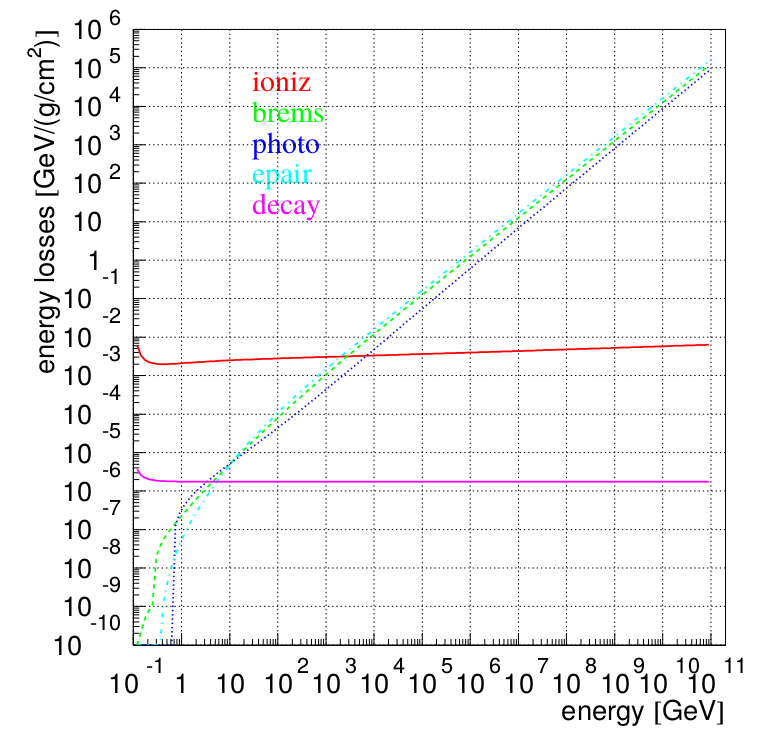
\includegraphics[width = 0.7\textwidth]{chapter4/img/muonenergyloss.png}
\caption{Muon energy loss from ionization (upper solid curve), bremsstrahlung (dashed), photonuclear (dotted), pair production (dashed-dotted) and decay (lower solid curve).}
\end{figure}
The average energy loss along the muon trajectory can be parametrized by 

\begin{equation}
\label{eq:energyloss}
- \frac{dE}{dx} = a + b \cdot E_\mu,
\end{equation}
where $a$ and $b$ are obtained by fitting and can be found in Table \ref{tab:fits} \footnote{Mwe stands for ``meter water equivalent'', a unit often used in cosmic ray physics. A detector shielded by matter equal to 100 mwe would be equally shielded from cosmic rays if it were 100 meters below water.} \ref{tab:energylossconstants}. The muon range can be found by integrating Eq. \ref{eq:energyloss}

\begin{equation}
\begin{split}
R_\mu \approx \frac{1}{b} \ln \left( \frac{E_\mu}{E_{th}} +1 \right),
\end{split}
\end{equation}
with $E_th = a/b = 720$ GeV, the energy theshold above which stochastic effects are dominant. 
% Please add the following required packages to your document preamble:
% \usepackage[table,xcdraw]{xcolor}
% If you use beamer only pass "xcolor=table" option, i.e. \documentclass[xcolor=table]{beamer}
\begin{table}[]
\label{tab:fits}
\centering
\begin{tabular}{|
>{\columncolor[HTML]{9B9B9B}}l |c|c|}
\hline
{\color[HTML]{000000} Medium}   & \cellcolor[HTML]{9B9B9B}{$a \left(\frac{\textrm{GeV}}{\textrm{mwe}}\right)$} & \cellcolor[HTML]{9B9B9B}{$b \left(\frac{10^{-3}}{\textrm{mwe}}\right)$} \\ \hline \hline
{\color[HTML]{000000} Air}      & 0.281                                                                                             & 0.347                                                                                        \\ \hline
{\color[HTML]{000000} Ice}      & 0.259                                                                                             & 0.363                                                                                        \\ \hline
{\color[HTML]{000000} Fr. Rock} & 0.231                                                                                             & 0.436                                                                                        \\ \hline
{\color[HTML]{000000} St. Rock} & 0.223                                                                                             & 0.463                                                                                        \\ \hline
\end{tabular}
\caption{Best fits for muon energy loss parameters $a$ and $b$ from Eq. \ref{eq:energyloss}. Fits from \cite{Chirkin:2004hz}.}
\end{table}


\section{Energy loss formulae}
\label{sec:energyloss}
Zie thesis Dima en PPC paper.
\subsection{Ionization}
Bethe Bloch
\begin{figure}
\label{fig:ICinteractions}
\centering
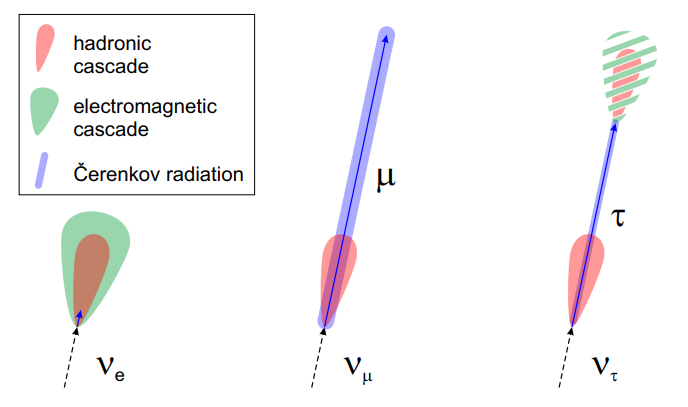
\includegraphics[width=0.7\textwidth]{chapter4/img/ICinteractions.png}
\caption{Schematic view of the neutrino signatures in matter. At each interaction point there is a hadronic cascade (red). Every hadronic cascade has electromagnetic sub-showers which are not illustrated here. Muons and energetic taus can give rise to tracks. Illustrations from \cite{Wallraff}.}
\end{figure}

